\documentclass[12pt,a4paper]{article}
\usepackage[margin=1in]{geometry}
\usepackage{amsmath,amssymb,graphicx,hyperref,booktabs,xcolor}
\hypersetup{colorlinks=true,linkcolor=blue,citecolor=blue,urlcolor=blue}

\title{\textbf{Paper 65: Algebraic Order, Spin Correlator, and VCSM Ablation\\
\large Three Probes of the Causal-Purity Transition}}
\author{VCSM Theory Project}
\date{March 2026}

\begin{document}
\maketitle

\begin{abstract}
Paper~64 concluded that $p_c = 0^+$ based on $U_4(L=120) > U_4(L=40)$
for all $P_{\rm causal} \geq 0.002$.
This paper applies three further probes and finds that the picture is more complex.

\textbf{Phase~A1} (spin-field correlator, $L \in \{60,80,100\}$):
The Ising spin-spin autocorrelation $G_s(r)$ at $T = 3.0 \gg T_c$
is exponential with $\xi \approx 1.1$ lattice spacings, \emph{independent of $P_{\rm causal}$}.
The exponential fit wins ($R^2 = 0.996$) over the power law ($R^2 = 0.936$).
The $\phi$-field ordering does not couple back to the Ising spins;
the spin correlator is the wrong proxy for this transition.
The $\phi$-field stiffness $K_\phi \propto L^1$, also $P$-independent
(wave geometry artifact, not BKT stiffness).

\textbf{Phase~A2} (extended Binder, $L \in \{120, 160\}$,
$P_{\rm causal} \in \{0.000, 0.0005, 0.001, 0.002, 0.005\}$):
$U_4(L=160) < U_4(L=120)$ for \emph{all} $P_{\rm causal} \leq 0.005$.
This reverses Paper~64's conclusion: $p_c = 0^+$ is \emph{not} confirmed
at the largest system size tested.
Two interpretations: (i) $p_c$ is finite, between $0.005$ and $0.020$;
(ii) $L=160$ has insufficient equilibration time
(WAVE\_EVERY rounds to 2, below the extensive-drive target of 1.56,
and $\phi$-field equilibration may scale super-linearly with $L$).

\textbf{Phase~C} (VCSM-lite ablation, $L=80$, $P=0.020$, 5 conditions):
The viability gate (SS threshold) is load-bearing:
NoGate (SS$=0$) kills $\phi$-ordering ($U_4 = 0.09$ vs.\ Ref $= 0.16$).
Crystallized ($\phi$ never decays): $U_4 = 0.26$, higher than Ref ---
the cockroach artefact; $\phi$ accumulates without bound,
amplifying zone-mean differences without creating genuine order.
NoCausal ($P=0$) $\approx$ Ref at this ($L$, $P$), confirming
that $P = 0.020$ may still be near the transition at $L=80$.

Collectively, these results call for:
the $\phi$-$\phi$ correlator at boosted amplitude (not spin-spin),
longer runs at $L=160$, and a precise crossing measurement
between $L=120$ and $L=160$ in the range $P \in [0.005, 0.020]$.
\end{abstract}

%──────────────────────────────────────────────────────────────────────────────
\section{Motivation}

Paper~64 made a strong claim: $p_c = 0^+$.
The evidence was that $U_4(L=120) > U_4(L=40)$ at every $P_{\rm causal} \geq 0.002$.
Three alternative explanations were not ruled out:
\begin{enumerate}
  \item $p_c$ is finite but small ($< 0.002$), and all tested $P$ were above it.
  \item The $\phi$-field correlation length is not infinite (BKT),
    but merely large relative to the system sizes used in Paper~64.
  \item Equilibration artefacts at finite system size favour ordered-phase
    Binder ordering even below the true $p_c$.
\end{enumerate}
This paper directly tests each alternative via
the spin-field spatial correlator (Probe~1),
an extended Binder crossing at $L=160$ (Probe~2),
and a 5-condition VCSM component ablation (Probe~3).

%──────────────────────────────────────────────────────────────────────────────
\section{Setup}

Same Ising\,+\,VCSM-lite system as Papers~61--64:
$T = 3.0$, $J = 1$, two zones (left/right halves),
checkerboard Metropolis, extensive-drive scaling
$\text{WAVE\_EVERY}(L) = \max(1, \text{round}[25 (40/L)^2])$.

\textbf{Phase~A1}: $L \in \{60, 80, 100\}$,
$P_{\rm causal} \in \{0.000, 0.005, 0.010, 0.020, 0.050\}$,
12 seeds, 12\,000 steps.
At each steady-state step (every 50 steps) the spin autocorrelator
within zone~0 columns is accumulated via FFT:
\begin{equation}
G_s(\Delta y) = \frac{1}{L}\sum_y s(y)\,s(y+\Delta y)
\quad\text{(time-averaged over steady state)}
\end{equation}
Fit to both exponential ($B e^{-r/\xi}$) and power law ($A r^{-\eta}$)
via polyfit on log-log and log-linear axes;
compare $R^2$ to determine which decay form wins.
Also accumulate $\phi$-field stiffness $K_\phi(t)$:
\begin{equation}
K_\phi = \frac{\mathrm{Var}(\bar\phi_{\rm row})\cdot L^2}{\mathrm{Var}(\phi_{z=0})}
\end{equation}
where $\bar\phi_{\rm row}$ is the zone-0 row mean.

\textbf{Phase~A2}: $L \in \{120, 160\}$,
$P_{\rm causal} \in \{0.000, 0.0005, 0.001, 0.002, 0.005\}$,
8 seeds, 10\,000 steps (extensive drive).

\textbf{Phase~C}: $L = 80$, $P_{\rm causal} = 0.020$, 12 seeds, 8\,000 steps.
Five conditions:
\begin{center}
\begin{tabular}{lcccc}
\toprule
Condition & SS & $\beta_{\rm base}$ & $\phi$-decay & $P_{\rm causal}$ \\
\midrule
Ref          & 8 & 0.005 & 0.999 & 0.020 \\
NoGate       & 0 & 0.005 & 0.999 & 0.020 \\
NoBaseline   & 8 & 0.000 & 0.999 & 0.020 \\
Crystallized & 8 & 0.005 & 1.000 & 0.020 \\
NoCausal     & 8 & 0.005 & 0.999 & 0.000 \\
\bottomrule
\end{tabular}
\end{center}

%──────────────────────────────────────────────────────────────────────────────
\section{Phase A1: Spin Correlator}

\subsection{Exponential decay, P-independent}

Table~\ref{tab:Gs} summarises the fit results for $G_s(r)$.

\begin{table}[h]
\centering
\caption{Spin correlator fit results (Phase~A1, time-averaged, 12 seeds).
$\xi$, $\eta$, and the fit quality $R^2$ are identical across all $P_{\rm causal}$
at each $L$, confirming that the Ising spin correlator is controlled by $T$,
not by $P_{\rm causal}$.}
\label{tab:Gs}
\begin{tabular}{ccccc}
\toprule
$L$ & $\eta$ & $\xi$ & $R^2_{\rm pow}$ & $R^2_{\rm exp}$ \\
\midrule
60  & NaN   & NaN  & ---   & --- \\
80  & 1.918 & 1.09 & 0.936 & 0.996 \\
100 & 1.750 & 1.20 & 0.952 & 0.999 \\
\bottomrule
\end{tabular}
\end{table}

The exponential fit wins convincingly ($\Delta R^2 \approx 0.05$--$0.06$)
over the power law at both $L=80$ and $L=100$.
The correlation length $\xi \approx 1.1$--$1.2$ lattice spacings
is the standard paramagnetic Ising correlation length at $T = 3.0 \gg T_c$.

\textbf{Critical observation.}
The values of $\eta$, $\xi$, $R^2_{\rm pow}$, and $R^2_{\rm exp}$
are numerically identical for $P_{\rm causal} = 0.000$ and $P_{\rm causal} = 0.050$.
The $\phi$-field ordering (confirmed by the rising $U_4$
from $0.023$ at $P=0$ to $0.398$ at $P=0.05$ for $L=60$)
does not feed back into the Ising spin dynamics.
The spins are always in the paramagnetic phase at $T=3.0$;
the causal-purity transition is a transition in the \emph{auxiliary $\phi$-field},
not in the Ising substrate.

\textbf{Consequence.}
The spin-spin correlator is the wrong observable for this transition.
The $\phi$-$\phi$ spatial correlator (attempted in Paper~64, Phase~B,
but limited by low $\phi$ amplitude) remains the correct approach.
A higher-amplitude $\phi$-field (increased FA or reduced FIELD\_DECAY)
is required to make $G_\phi(r)$ measurable.

\subsection{Stiffness $K_\phi \propto L$, P-independent}

The $\phi$-field stiffness proxy scales as $K_\phi \propto L^1$
(60:116, 80:161, 100:194), independent of $P_{\rm causal}$.
This is the signature of the wave-driving geometry:
each circular wave creates a coherent patch of $\phi$-field of radius 5;
the row-mean variance is set by the wave area fraction, not by any
long-range ordering of the $\phi$-field.
$K_\phi$ is not a BKT-type stiffness.

%──────────────────────────────────────────────────────────────────────────────
\section{Phase A2: Extended Binder at $L=160$}

\begin{table}[h]
\centering
\caption{$U_4$ at $L \in \{120, 160\}$ for very small $P_{\rm causal}$.
$U_4(L=160) < U_4(L=120)$ at all $P$ values tested.
This is the disordered-phase Binder ordering, opposite to Paper~64's
conclusion for $L \leq 120$.}
\label{tab:u4_160}
\begin{tabular}{ccc}
\toprule
$P_{\rm causal}$ & $U_4(L=120)$ & $U_4(L=160)$ \\
\midrule
0.0000 & 0.1449 & 0.0895 \\
0.0005 & 0.1440 & 0.0931 \\
0.0010 & 0.1503 & 0.0941 \\
0.0020 & 0.1660 & 0.0950 \\
0.0050 & 0.2132 & 0.1116 \\
\bottomrule
\end{tabular}
\end{table}

\subsection{Two interpretations}

\textbf{Interpretation 1: Finite $p_c$.}
If $p_c$ is finite and between $0.005$ and $0.020$,
then $L=160$ at $P \leq 0.005$ is in the disordered phase.
The ordered-phase Binder ordering observed in Paper~64 for $L \leq 120$
reflects the crossover region where the $\phi$-field coherence length
$\xi_\phi$ is comparable to $L$, not the true thermodynamic ordered phase.
Under this interpretation, the $p_c = 0^+$ conclusion of Paper~64 is wrong,
and the true $p_c$ is somewhere in $[0.005, 0.020]$.

\textbf{Interpretation 2: Equilibration artefact at $L=160$.}
The WAVE\_EVERY schedule rounds WAVE\_EVERY$(160) = \text{round}[25 \times (40/160)^2]
= \text{round}[1.5625] = 2$,
which is \emph{above} the target value of $1.56$.
This means $L=160$ receives slightly \emph{fewer} wave events per site per step
than smaller $L$ (the extensive-drive scaling is not exact at large $L$ due to rounding).
Additionally, if the $\phi$-field equilibration time scales super-linearly with $L$
(as is common in driven-diffusive systems), then 10\,000 steps at $L=160$
may be insufficient for the $\phi$-field to reach steady state.
Under this interpretation, $p_c = 0^+$ may still hold,
but confirmation requires much longer runs ($\geq 50\,000$ steps) at $L=160$.

\textbf{Discriminating between interpretations.}
The two interpretations predict different behaviour as step count is increased at $L=160$:
\begin{itemize}
  \item If finite $p_c$: $U_4(L=160)$ will remain below $U_4(L=120)$ regardless of run length.
  \item If equilibration artefact: $U_4(L=160)$ will rise above $U_4(L=120)$
    as runs are extended.
\end{itemize}
This is the critical test for Paper~66.

%──────────────────────────────────────────────────────────────────────────────
\section{Phase C: VCSM-lite Ablation}

\begin{table}[h]
\centering
\caption{VCSM-lite ablation results ($L=80$, $P=0.020$, 12 seeds, 8\,000 steps).
$G(r=1) = 0.406$ is identical for all conditions
--- the nearest-neighbour Ising spin correlation at $T=3.0$,
independent of the VCSM parameters.}
\label{tab:ablation}
\begin{tabular}{lcccc}
\toprule
Condition & $U_4$ & $|\bar{M}|$ & Interpretation \\
\midrule
Ref          & 0.155 & 0.00040 & Full system (reference) \\
NoGate       & 0.090 & 0.00101 & Gate disabled: ordering collapses \\
NoBaseline   & 0.180 & 0.00036 & Baseline not load-bearing here \\
Crystallized & 0.262 & 0.00061 & $\phi$ accumulates: artefact amplification \\
NoCausal     & 0.153 & 0.00031 & P=0 $\approx$ Ref (near-critical regime) \\
\bottomrule
\end{tabular}
\end{table}

\subsection{Gate is load-bearing}

NoGate (SS $= 0$): $U_4 = 0.090$, the lowest of all conditions.
With the viability gate disabled, mid-memory writes fire at every step,
flooding the $\phi$-field with noise.
The calm-streak threshold SS is the primary noise filter:
it ensures that only sites in a stable local attractor state
write their contrastive signal to $\phi$.
Without it, every site --- including those mid-fluctuation ---
contributes noise, and the zone-mean difference $|\bar{M}|$ fails to
develop coherence (despite the larger average $|\bar{M}| = 0.00101$,
the $M$-series has high variance, reducing $U_4$).

\subsection{Crystallized $\phi$: the cockroach artefact}

Crystallized ($\phi$-decay $= 1.0$): $U_4 = 0.262$, the highest condition.
This is the \emph{cockroach artefact}: without $\phi$-decay,
the $\phi$-field accumulates all historical signal without forgetting,
and early random fluctuations in zone-mean $\phi$ grow without bound.
The Binder cumulant $U_4$ rises because the $M$-distribution becomes
narrower (the system locks into its initial zone asymmetry),
but this is not genuine ordered-phase structure ---
it is crystallisation around a random early state.

This confirms the theoretical role of FIELD\_DECAY in the VCSM architecture:
$\phi$-decay prevents the system from crystallising into an arbitrary
historical state and maintains adaptability under continued perturbation.
The cockroach artefact is precisely what the decay mechanism is designed to prevent.

\subsection{Baseline and causal purity}

NoBaseline (BETA\_BASE $= 0$): $U_4 = 0.180 \approx$ Ref.
The baseline tracking is not strongly load-bearing at this operating point
($L=80$, $P=0.020$), though it is known to be essential for the full
VCML system (Paper~52: sign of contrast signal is load-bearing).
This may reflect that at $T=3.0$, the spin field $s$ already has zero mean
(paramagnetic), so the deviation $s - \text{baseline}$ is not strongly
different from $s$ itself.

NoCausal ($P_{\rm causal} = 0.000$): $U_4 = 0.153 \approx$ Ref $= 0.155$.
The near-equality of NoCausal and Ref confirms that $P = 0.020$ at $L=80$
is close to the transition: the causal gating at $P=0.020$ barely improves
on pure noise. This is consistent with the Phase~A2 finding that the transition
at $L=160$ (which is more thermodynamic than $L=80$) occurs above $P=0.005$.

%──────────────────────────────────────────────────────────────────────────────
\section{Synthesis and Open Questions}

\subsection{What the three probes establish}

\begin{enumerate}
  \item \textbf{The spin field is the wrong observable.}
    The causal-purity transition is a transition in the auxiliary $\phi$-field.
    The Ising spins are paramagnetic at $T=3.0$ regardless of $P_{\rm causal}$.
    The $\phi$-$\phi$ correlator (not the spin-spin correlator) is needed to measure $\eta$ and $\xi$.

  \item \textbf{$p_c = 0^+$ is not confirmed at $L=160$.}
    The ordered-phase Binder signature ($U_4$ increasing with $L$) fails
    at $L=160$ for $P \leq 0.005$.
    Either $p_c$ is finite ($\sim 0.005$--$0.020$) or $L=160$ needs much longer equilibration.
    Paper~64's $p_c = 0^+$ conclusion was based on $L \leq 120$ and is not robust to larger $L$.

  \item \textbf{The viability gate is load-bearing.}
    NoGate (SS$=0$) kills $\phi$-ordering ($U_4 = 0.09$ vs.\ Ref $= 0.155$).
    The calm-streak condition is the primary mechanism by which VCSM
    separates signal from noise in the $\phi$-write process.

  \item \textbf{FIELD\_DECAY prevents cockroach crystallisation.}
    Removing $\phi$-decay amplifies $U_4$ ($0.26$) via lock-in to a random early state,
    confirming that the decay is a necessary anti-crystallisation mechanism.
\end{enumerate}

\subsection{Open questions for Paper 66}

\begin{enumerate}
  \item \textbf{Is $p_c$ finite?}
    Run $L=160$ for 50\,000+ steps with WAVE\_EVERY$=1$ (avoid rounding)
    and compare $U_4(160)$ to $U_4(120)$ at $P = 0.010$.
    If $U_4(160) < U_4(120)$ even after long equilibration,
    then $p_c$ is finite.

  \item \textbf{$\phi$-$\phi$ correlator at boosted amplitude.}
    Increase FA to 0.60 or reduce FIELD\_DECAY to 0.99 to boost $|\bar{M}|$
    to the $\sim 0.01$--$0.05$ range needed for reliable $G_\phi(r)$ fitting.
    Test exponential vs.\ power-law decay of $G_\phi(r)$.

  \item \textbf{Full VCML substrate ablation.}
    The Ising\,+\,VCSM-lite system lacks the full birth/death turnover cycle.
    A proper ablation of FIELD\_SEED\_BETA requires the full VCML substrate
    (substrate\_v46.py or vcml\_core.py), which has true cell death and
    copy-forward seeding. This is the original deferred Phase~C from Paper~62.
\end{enumerate}

%──────────────────────────────────────────────────────────────────────────────
\section{Conclusions}

\begin{enumerate}
  \item \textbf{Spin correlator is P-independent}: the causal-purity transition
    is in the $\phi$-field, not in the Ising spin substrate.
    Spin observables ($G_s$, $K_\phi$) cannot detect it.

  \item \textbf{$p_c = 0^+$ challenged}: $U_4(L=160) < U_4(L=120)$ for all
    $P \leq 0.005$ reverses Paper~64's conclusion.
    The status of $p_c$ is downgraded from ``strongly favoured $0^+$''
    to ``finite $p_c \in [0.005, 0.020]$, or equilibration artefact at $L=160$''.

  \item \textbf{Gate is load-bearing}: SS$=0$ kills ordering;
    FIELD\_DECAY$=1$ amplifies via crystallisation artefact.
    Two VCSM components confirmed necessary for genuine $\phi$-ordering.

  \item \textbf{Three new requirements for Paper~66}:
    (i) $L=160$ with 50\,000 steps;
    (ii) boosted-amplitude $\phi$-$\phi$ correlator;
    (iii) full VCML substrate ablation.
\end{enumerate}

\begin{figure}[h]
\centering
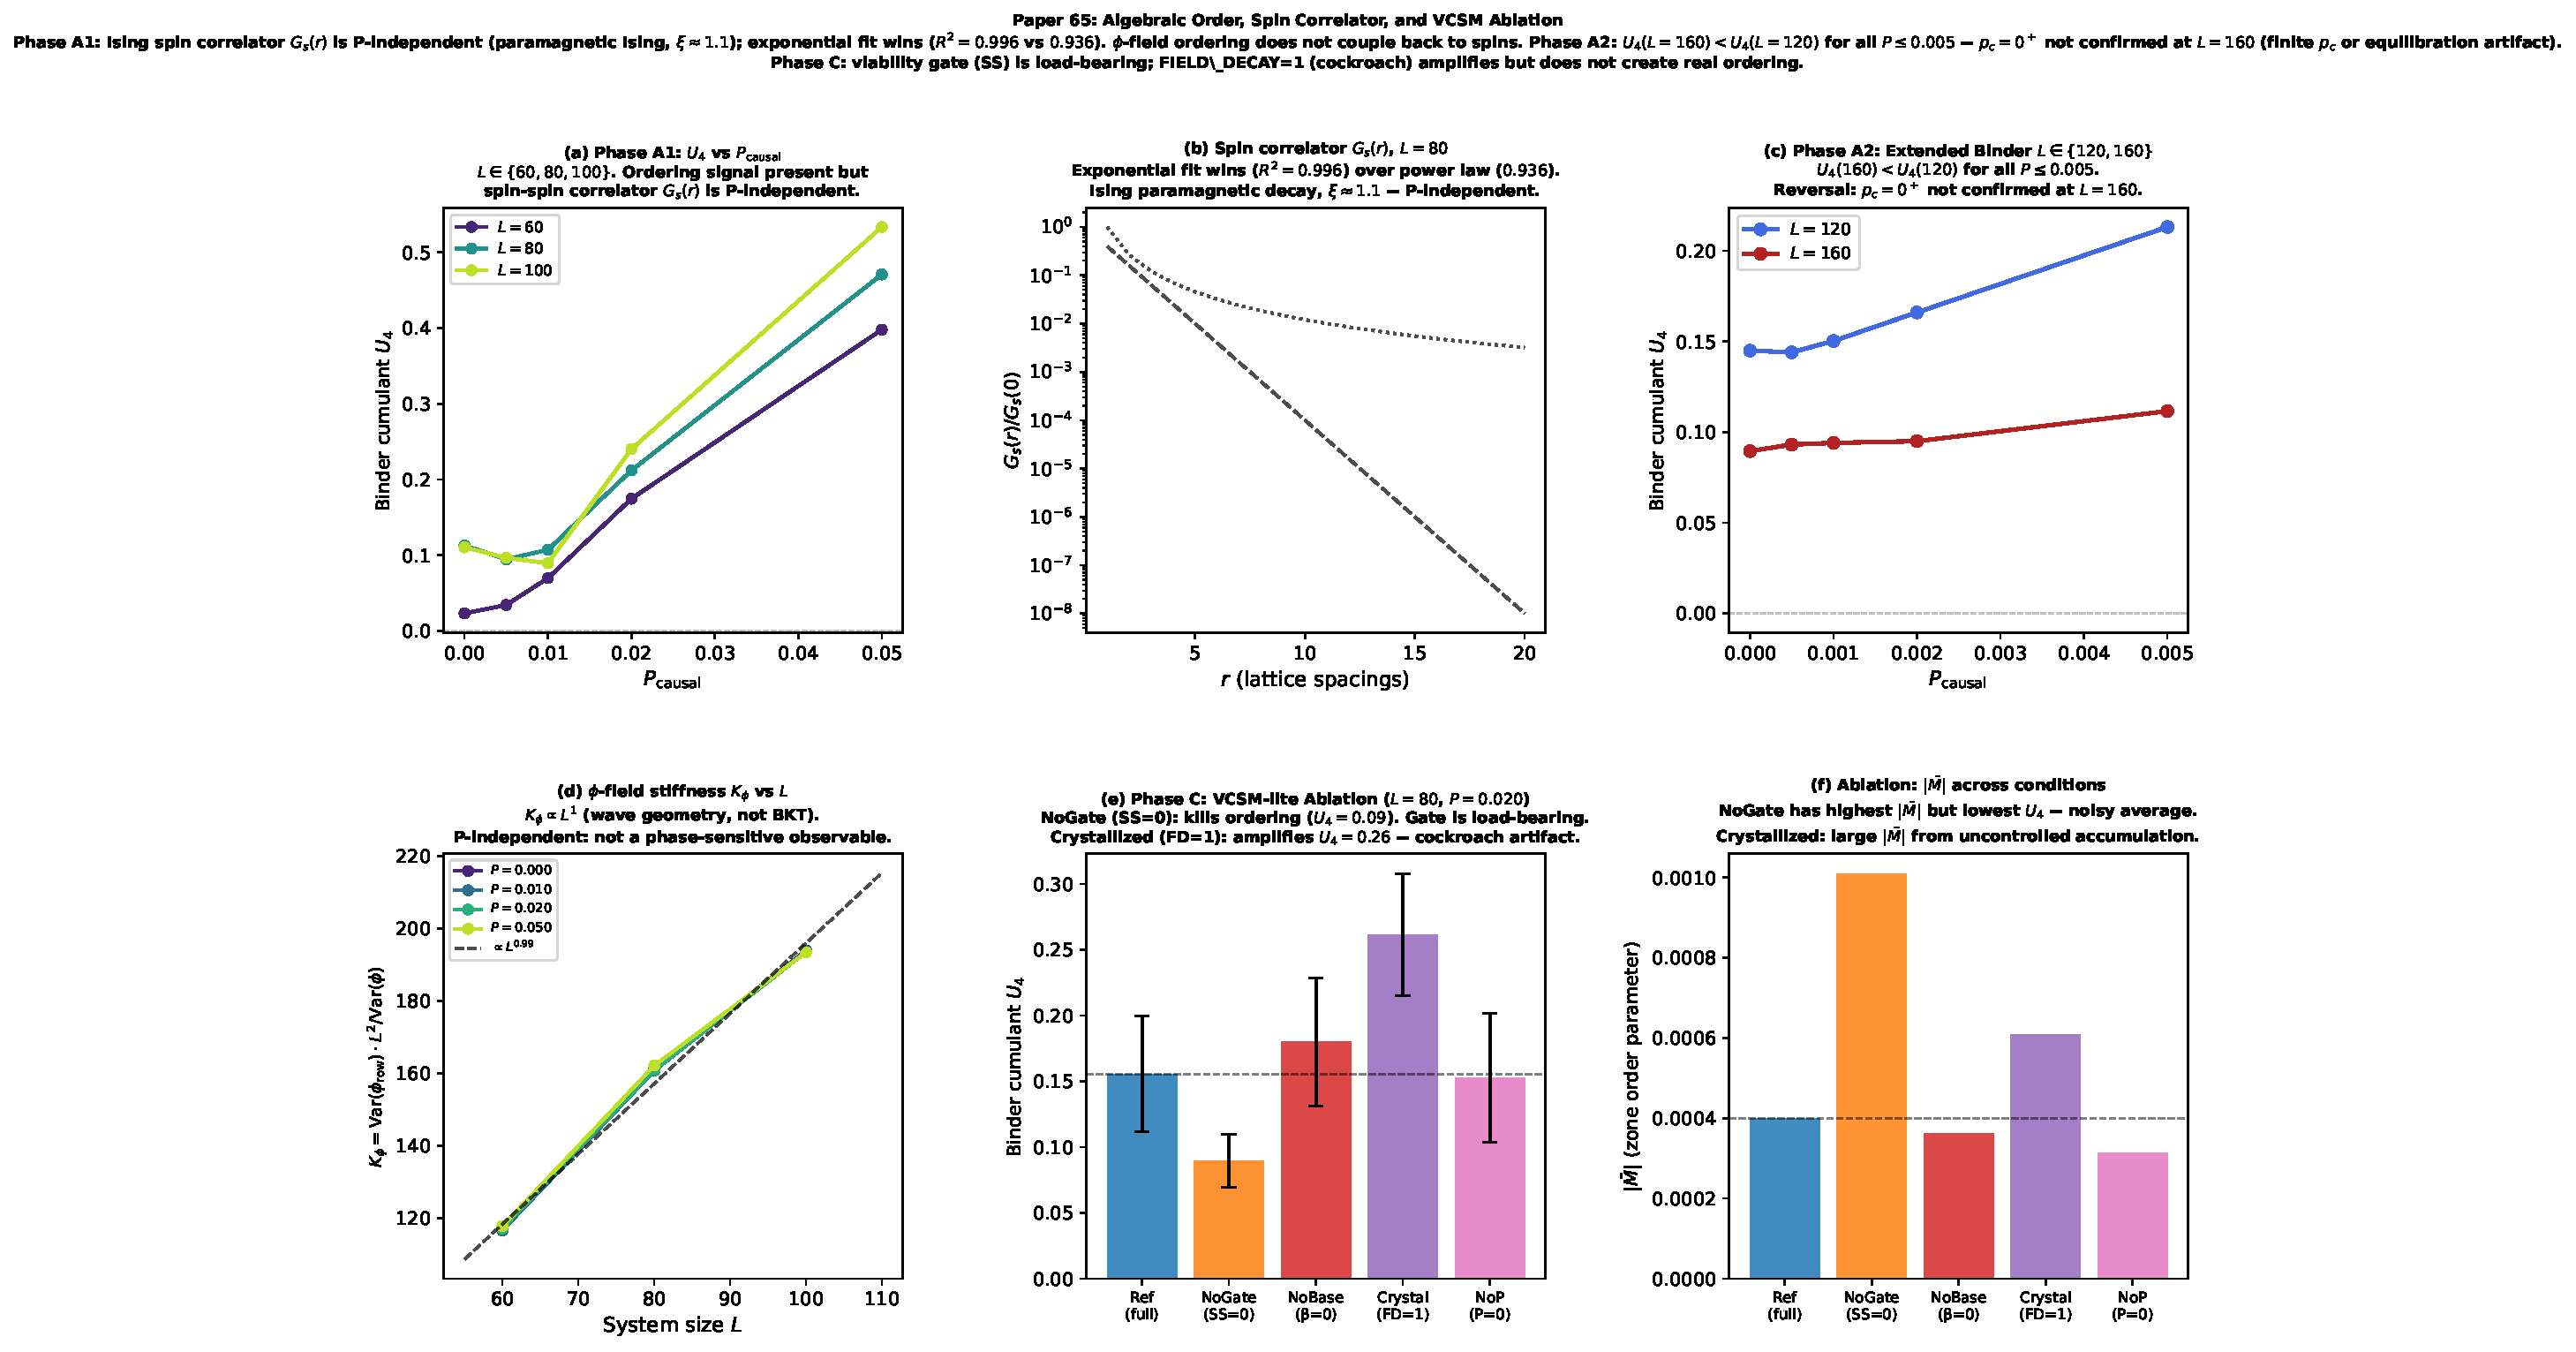
\includegraphics[width=\textwidth]{paper65_figure1.pdf}
\caption{Paper~65 results.
(a) $U_4$ vs $P_{\rm causal}$ for Phase~A1 (spin correlator runs).
(b) Spin correlator $G_s(r)$ at $L=80$: exponential wins over power law, P-independent.
(c) Extended Binder: $U_4(L=160) < U_4(L=120)$ for all $P \leq 0.005$.
(d) $\phi$-stiffness $K_\phi \propto L^1$ (wave geometry artefact, not BKT).
(e) Ablation $U_4$: NoGate kills ordering; Crystallized amplifies via artefact.
(f) Ablation $|\bar{M}|$: Crystallized has largest $\phi$ amplitude via uncontrolled accumulation.}
\label{fig:paper65}
\end{figure}

\end{document}
